\chapter{Modelo matemático}

De acuerdo con \cite[p.~14]{Dombre2007}, el diseño y control de robots requiere diversos modelos matemáticos, tales como:

\begin{itemize}
\item Cinemática directa e inversa, es decir, encontrar la posición del efector final en términos de las coordenadas de las articulaciones y viceversa.
\item Cinemática de la velocidad, encontrar la velocidad del efector final en términos de la velocidad de las articulaciones y viceversa.
\item Modelo dinámico, el cual establece la relación entre los torques o fuerzas que ejercen los actuadores y las posiciones, velocidades y aceleraciones de las articulaciones.
\end{itemize}

\begin{figure}
    \centering
    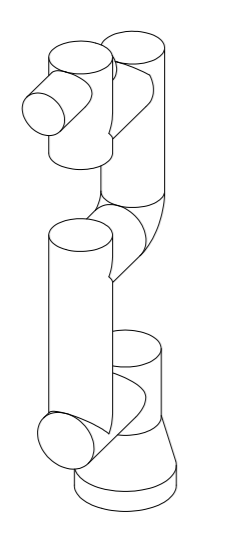
\includegraphics[scale=0.7]{./img/chapter4/robotarmprototype.png}
    \caption{Boceto del brazo robótico propuesto}
    \label{fig:roboticarmprototype}
\end{figure}

En este capítulo se desarrollarán estos modelos matemáticos, los cuales son necesarios para simular y predecir el comportamiento del mismo. 

Para realizar estos modelos, es necesario contar con los parámetros físicos y geométricos del robot, los cuales, para una primera aproximación se mencionarán a continuación.

%Insertar tabla de dimensiones y parámetros

Otros requerimientos necesarios para el desarrollo del modelo matemático es el alcance total del brazo, el cual deberá ser de mínimo 500 mm, la velocidad, la cuál deberá estar en un rango entre 5 RPM y 30 RPM, y por último, la carga útil deberá ser de 2 kg.

En la figura \ref{fig:roboticarmprototype} podemos ver un boceto del brazo robótico que se planea implementar.

Con estos datos claros, es posible empezar la realización de los modelos matemáticos.

\section{Cinemática directa e inversa}
\subsection{Cinemática directa}

La cinemática directa de un robot se refiere al cálculo de la posición y orientación del marco de referencia del efector final desde sus coordenadas $\theta$. \cite{University2017}

\subsubsection{Matriz de transformación homogénea}

Según \cite{University2017}, existen tres usos principales para una matriz de transformación homogénea:

\begin{enumerate}
  \item Para representar la configuración (posición y orientación) de un cuerpo rígido.
  \item Para cambiar el marco de referencia en el cuál está representado un vector o un \textit{frame}.
  \item Para desplazar un vector o un \textit{frame}.
\end{enumerate}

Para el caso que nos ocupa, necesitamos la matriz de transformación homogénea desde la base fija del robot hasta su efector final, descrita con la ecuación siguiente:

\begin{equation}
\label{eq:forwardkinematicequation}
\begin{split}
{}_{0}^{7}T = \mathscr{T}_z(a_1)\oplus\mathscr{R}_z(\theta_1)\oplus\mathscr{T}_x(b_1)\oplus\mathscr{R}_x(\theta_2)\oplus\mathscr{T}_z(c_1)\oplus\mathscr{R}_x(\theta_3) \\ \oplus\mathscr{T}_z(d_1)\oplus\mathscr{T}_x(d_2)\oplus\mathscr{R}_x(\theta_4)\oplus\mathscr{T}_x(e_1)\oplus\mathscr{R}_z(\theta_5)\oplus\mathscr{T}_z(f_1)\oplus\mathscr{R}_x(\theta_6)
\end{split}
\end{equation}

\begin{figure}
    \centering
    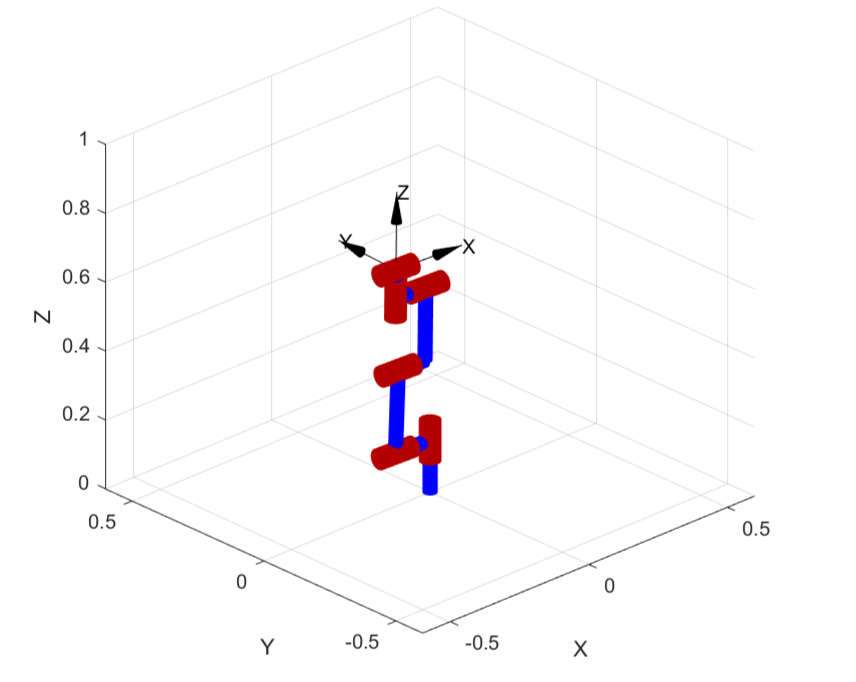
\includegraphics[scale=0.6]{./img/chapter4/KinematicDiagramML.png}
    \caption{Cadena cinemática}
    \label{fig:kinematicchain}
\end{figure}


En la imagen \ref{fig:kinematicchain} podemos observar la cadena cinemática de nuestro brazo robótico, fue creada con un algoritmo en MATLAB con ayuda de la herramienta Robotic Toolbox, desarrollada por Peter Corke \cite{Corke2017}, dicho código puede consultarse en el Anexo 1.





\subsubsection{Convención de Denavit-Hartenberg}


\begin{table}[h]
\centering
\caption{Parámetros Denavit Hartenberg}
 \label{table:denavithartenberg}
\begin{tabular}{l|l|l|l|l|}
               & $\theta$ [rad] & a [m]    & d [m]   & $\alpha$ [rad]                        \\ 
\hline
Articulación 1 & 0                           & 0        & 0.1519  & $\frac{\pi}{2}$   \\
Articulación 2 & 0                           & -0.24365 & 0       & 0                                                  \\
Articulación 3 & 0                           & -0.21325 & 0       & 0                                                  \\
Articulación 4 & 0                           & 0        & 0.11235 & $\frac{\pi}{2}$   \\
Articulación 5 & 0                           & 0        & 0.08535 & $-\frac{\pi}{2}$  \\
Articulación 6 & 0                           & 0        & 0.0819  & 0                                                 
\end{tabular}
\end{table}

\subsection{Cinemática inversa}
No estoy seguro para que me servirá, si lo hará el software. MoveIt o MATLAB.

\section{Cinemática de la velocidad}


\section{Modelo dinámico}
\subsection{Formulación Lagraniana}
\subsection{Formulación Newton-Euler}